\documentclass[10pt]{beamer}

\usepackage[british]{babel}
\usepackage{graphicx}
\usepackage{hyperref}
\usepackage{uzh}
\usepackage{url}
\usepackage{booktabs}
\usepackage{amsmath}
\usepackage{bm}
\let\svthefootnote\thefootnote

%%% FOR DEFINITION BOX:
\usepackage{tcolorbox} % for theorem box
\tcbuselibrary{theorems}
%[number within=section]
%\newtcbtheorem{def}{Definition}{colback=green!5,colframe=green!35!black,fonttitle=\bfseries}{th}

\newtcbtheorem{def_box}{Definition}%
{colback=blue!5,colframe=blue!35!black,fonttitle=\bfseries}{th}

\definecolor{colortheme}{RGB}{0,87,163} 



% The title of the presentation:
%  - first a short version which is visible at the bottom of each slide;
%  - second the full title shown on the title slide;
\title[Deep Reinforcement Learning - A Portfolio Management Approach]{Deep Reinforcement Learning:\\ A Portfolio Management Approach}
% Optional: a subtitle to be dispalyed on the title slide
%\subtitle{An Introduction to Financial Econometrics}

% The author(s) of the presentation:
%  - again first a short version to be displayed at the bottom;
%  - next the full list of authors, which may include contact information;
\author[Polák, Lag, Lucescu]{ Jakub \textsc{Polák}\\
    Thomas \textsc{Lagos}\\
	Patrick \textsc{Lucescu}}

% The institute:
%  - to start the name of the university as displayed on the top of each slide
%    this can be adjusted such that you can also create a Dutch version
%  - next the institute information as displayed on the title slide
\institute[University of Zurich]{
	Deep Reinforcement Learning Seminar\\
	Drunk Policy}

% Add a date and possibly the name of the event to the slides
%  - again first a short version to be shown at the bottom of each slide
%  - second the full date and event name for the title slide
\date[]{\today}

\begin{document}

\begin{frame}
  \titlepage
\end{frame}

%%%%%%%%%%%%%%%%%%%%%%%%%%%%%%%%%%%%%%%%%%%%%%%%%%%%
%%% Theory
%%%%%%%%%%%%%%%%%%%%%%%%%%%%%%%%%%%%%%%%%%%%%%%%%%%%
% Section titles are shown in at the top of the slides with the current section 
% highlighted. Note that the number of sections determines the size of the top 
% bar, and hence the university name and logo. If you do not add any sections 
% they will not be visible.

%%%%%%%%%%%%%%%%%%%%% %%%%%%%%%%%%%%%%%%%%% %%%%%%%%%%%%%%%%%%%%% 
%%%%%%%%%%%%%%%%%%%%% %%%%%%%%%%%%%%%%%%%%% %%%%%%%%%%%%%%%%%%%%% 

\begin{frame}
\frametitle{Outline}
	\begin{enumerate}
		\item The Paper
		\item Our approach
		\begin{itemize}
		    \item Data 
		    \item Data Preprocessing
		    \item Reinforment Framework
		\end{itemize}
	\end{enumerate}
\end{frame}

%%%%%%%%%%%%%%%%%%%%%%%%%%%%%%%%%%%%%%%%%
%%%%%%%%%%%%%%%%%%%%%%%%%%%%%%%%%%%%%%%%%
\section{Context}
%%%%%%%%%%%%%%%%%%%%%%%%%%%%%%%%%%%%%%%%%


\begin{frame}{The Paper}
    \begin{itemize}
        \item In the paper "A Deep Reinforcement Learning Framework for the Financial Portfolio Management Problem", Zhengyao Jiang, Dixing Xu, Jinjun Liang present a financial-model-free Reinforcement Learning framework to provide a deep machine learning solution to the portfolio management problem.
        \item This is done on the context of cryptocurrencies markets using an Ensemble of Identical Independent Evaluators topology.
    \end{itemize}
\end{frame}

\begin{frame}{Our approach - Main Idea}
\begin{itemize}
    \item Our approach follows the lines of the above mentioned paper but we try to apply it in the context of traditional asset classes.
    \item Due to data constraints we also consider intraday trading
\end{itemize}
\end{frame}

\begin{frame}{Data}
\begin{itemize}
    \item Intraday data( preferably tick by tick) of main asset classes indexes 
    \item Liquidity requirements
    \item Still up to consideration due to data availability
\end{itemize}
\end{frame}



\begin{frame}{ Data Preprocessing}
\begin{itemize}
    \item We follow the same preprocessing as the main paper.
    \item For each stock, the input is a raw time series of the prices (High, Low, Open, Close) for a given period of time which is prespecified.
    \item The output is a matrix of 4 rows and n (number of available data points) columns.
    \item Columns correspond to:
    \begin{enumerate}
        \item Close(t-1)/Open(t-1)
        \item High(t-1)/Open(t-1)
        \item Low(t-1)/Open(t-1)
        \item Open(t)/Open(t-1)
    \end{enumerate}
\end{itemize}
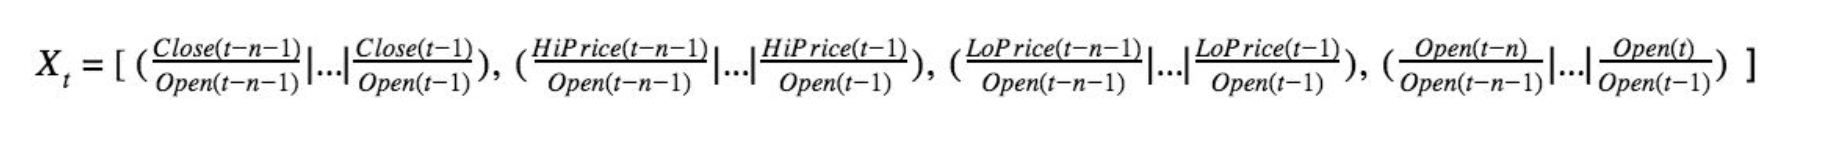
\includegraphics[width=\textwidth]{Presentation/inputTensor.png}
\end{frame}

\begin{frame}{Reinforcement Learning Setting}
\begin{itemize}
    \item The state at time t is the input matrix and the previous portfolio weights (at time t-1)
    \item The action is the vector of investment weight (at time t).
    \item The reward function is defined such as it is the agent's return minus a baseline’s return (baseline is an eqully weighted agent - invest in all the possible stocks in the same way) minus a term estimating the transaction costs minus a proportion of the maximum weight difference between the weights at time t-1 and at time t
\end{itemize}
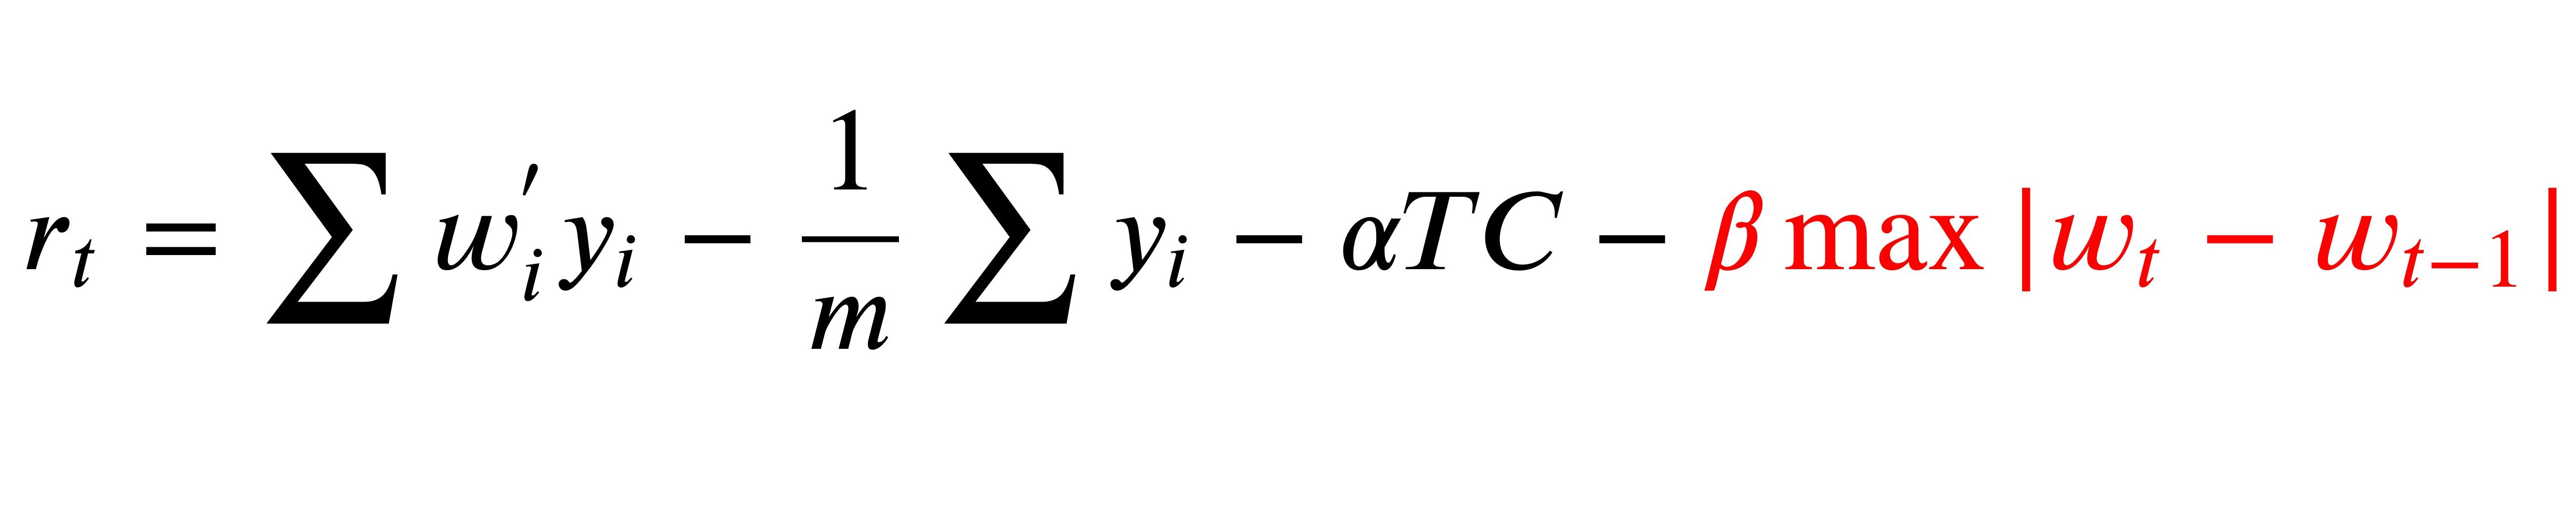
\includegraphics[width=\textwidth]{Presentation/r_tt.jpg}
    
\end{frame}

\begin{frame}{Reinforcement Learning Method}
\begin{itemize}
    \item policy gradient 
    \item the policy function is modelled by a neural network which takes as input the preprocessed data and the previous weights and outputs the new set of weights
\end{itemize}

\end{frame}

\begin{frame}{Reference}
\begin{itemize}
    \item \href{url}{https://arxiv.org/abs/1706.10059}
    \item \href{url}{https://github.com/ZhengyaoJiang/PGPortfolio}
    \item \href{url}{https://github.com/selimamrouni/Deep-Portfolio-Management-Reinforcement-Learning}
\end{itemize}
    
\end{frame}
\end{document}